\documentclass[manuscript,screen,review]{acmart}
\acmJournal{TECS}
\setcopyright{none}
\settopmatter{printacmref=false}
\usepackage{tikz}
\usetikzlibrary{arrows.meta,positioning}
\usepackage{tabularx}
\graphicspath{{figures/}}
\newcommand{\E}{\mathbb{E}}
\newcommand{\bits}{\mathcal{B}}
\newcommand{\risk}{R}
\newcommand{\ind}{\mathbf{1}}
\newcommand{\CE}{\operatorname{CE}}
\newcommand{\AUC}{\operatorname{AUC}}
\newcommand{\MSE}{\operatorname{MSE}}
\newcommand{\clip}{\operatorname{clip}}
\newtheorem{proposition}{Proposition}
% Expandable input for generated rows inside a booktabs alignment.
\makeatletter
\newcommand{\tablerows}[1]{\@@input #1 }
\makeatother

\title[NetSuRF: Evaluating Selective Bit Protection]{NetSuRF: A Bit-Accurate Evaluation of Selective Protection in Quantized Neural Networks}
\author{Manuel Blanco Valent\'{i}n}
\affiliation{\institution{Northwestern University}\city{Evanston}\state{Illinois}\country{USA}}
\author{Houxuan Guo}
\affiliation{\institution{Northwestern University}\city{Evanston}\state{Illinois}\country{USA}}
\author{Xiuyuan He}
\affiliation{\institution{Northwestern University}\city{Evanston}\state{Illinois}\country{USA}}
\author{Seda Ogrenci}
\affiliation{\institution{Northwestern University}\city{Evanston}\state{Illinois}\country{USA}}
\renewcommand{\shortauthors}{Blanco Valent\'{i}n et al.}
\keywords{quantized neural networks, encoded-bit faults, susceptibility estimation, selective protection, paired fault injection, embedded machine learning}

\begin{document}
\begin{abstract}
Selective protection of a quantized neural network requires deciding which stored bits merit a limited protection budget. A bit that is damaging in isolation need not have the largest protection value when other bits can fail simultaneously. NetSuRF evaluates this decision through a software flow connecting exact encoded-bit perturbations, susceptibility estimates, fixed-cardinality protection masks, paired fault fields, and application metrics. We study frozen INT8 ResNet-8 image classification, DS-CNN keyword spotting, and ToyCar anomaly detection using authoritative TensorFlow Lite reference inference. Six static policies are compared over logical bit-flip probabilities and protection budgets; gradient rankings use separately identified differentiable companions. At a logical bit-flip probability of $10^{-2}$ and 12.5\% protection, per-example absolute-gradient ranking exceeds MSB-first by 33.01 accuracy percentage points on ResNet-8, but the corresponding keyword-spotting gain is 3.52 points and the ToyCar ROC-AUC difference is inconclusive. These are fixed-model exploratory results, not evidence of universal superiority. A keyword-spotting comparison of published-form FKeras shows useful partial-tier allocation, complete-tier agreement with MSB-first, and no method dominating the grid. A separate targeted FP32 classifier study illustrates that loss and accuracy comparisons can differ, without establishing a general transformer result. An exact counterexample establishes the absence of a universal isolated-ranking guarantee. Bounded, independently evaluated allocation studies delimit its practical significance: no examined independent-pool arm resolves an improvement over exact isolated-bit allocation. Protection is ideal logical event suppression, and its cost is only the number of protected eligible bits. The contribution is a controlled, encoding-aware methodology for assessing ranking-to-protection decisions, including their failure modes and computational costs.
\end{abstract}
\ccsdesc[500]{Computer systems organization~Reliability}
\ccsdesc[300]{Computing methodologies~Neural networks}
\maketitle
\section{Introduction}
Quantized edge inference exposes a discrete reliability problem: changing one stored bit can change a parameter by a small step or reverse its sign with a large numerical jump. Protecting every parameter bit may be unnecessary for a particular application, but protecting only a fraction requires a defensible allocation rule. A practical software study must therefore connect a ranking to the task quality it preserves, not merely demonstrate that its scores correlate with a proxy for sensitivity.

We investigate the question: \emph{How reliably can static encoded-bit susceptibility rankings guide budget-constrained protection under simultaneous parameter faults?} Three distinctions are central. First, a numerical bit jump is not task damage. Second, an estimated derivative is not the finite effect of an encoded XOR. Third, damage measured with a single faulty bit is not generally the benefit of suppressing that bit when other bits may also be faulty. A ranking can be informative at one stage and disappointing at the next.

NetSuRF addresses these distinctions through an end-to-end software evaluation flow. It binds a frozen quantized model and dataset to an exact eligible bit population; constructs susceptibility scores and protection masks; applies matched persistent fault fields; and reports task metrics and computational cost. The tested protection operation perfectly suppresses proposed events on selected coordinates. Its budget is the number or fraction of eligible bits selected. This is a controlled logical comparison, not an implementation or cost model for a physical mitigation mechanism. Throughout the paper, a reliability curve means application quality under the specified logical fault distribution, not a device failure rate.

Our earlier FCCM work introduced a selective-protection design flow and a qualitative gradient/delta-based technique~\cite{guo2025inpixel}. The present study does not claim that flow as new. It isolates and evaluates the \emph{software ranking-to-allocation decision}: frozen INT8 codes, corrected baselines, authoritative faulted inference, common random fields, explicit task metrics, and independent evaluation of bounded allocation choices. The published FKeras method is evaluated alongside significance and first-order baselines, preserving its tier-first allocation rule.

The contributions are threefold. (1) An encoding-aware evaluation methodology separates numerical fault semantics, surrogate scores, ordering policies, and measured protection outcomes. (2) A controlled comparison across image classification, keyword spotting, and anomaly detection measures isolated-damage association, task quality versus BER and coverage, and score-construction cost, including unfavorable results. (3) A compact analytical and empirical assessment explains why isolated rankings lack a universal allocation guarantee while quantifying how little current bounded-pool evidence establishes about improvement over an exact isolated reference. The underlying probability identities are established mathematical tools, not newly invented foundations.

The findings support conditional engineering guidance rather than a universal winner. Per-example absolute gradients substantially outperform MSB-first on some ResNet-8 conditions; keyword-spotting gains are smaller, and ToyCar results depend strongly on budget and task metric. A ranking that predicts reconstruction MSE is not thereby validated for ROC-AUC protection. Likewise, a numerically validated Hessian score cannot be credited with effectiveness when the tested budget produces the same mask as MSB-first. These distinctions define both the useful results and the limits of this internal study.

\section{Related Work and Scope of the Contribution}
\paragraph{Sensitivity-guided fault analysis.}
FKeras combines sensitivity analysis, fault injection, and selective protection using a projection derived from leading weight-Hessian eigenpairs~\cite{weng2024fkeras}. Its bit-tier-first ordering is an important baseline, not a diagonal-Hessian approximation: a full weight Hessian includes cross-parameter curvature. PrioriFI uses Hessian-informed initialization and measured degradation to prioritize subsequent injections~\cite{weng2026priorifi}. EISFINN assigns attribution-based sampling weights to neuron outputs and bits to find critical faults efficiently~\cite{colucci2024eisfinn}. These works establish that informed fault selection and bit prioritization are not new. Their discovery objectives do not automatically equal expected risk of a fixed protection mask under a prescribed simultaneous-fault distribution.

Progressive bit-flip attacks already exploit quantized weight encoding and gradient-guided, state-updating search~\cite{rakin2019bfa}. Their deliberately chosen damaging flips differ from independent Bernoulli events. Worst-case attack outcomes cannot be used as unweighted estimates of the latter expectation. Our experiments do not compare attack success rates or introduce an adversarial sampler.

\paragraph{Selective protection and contextual effects.}
Su et al. use DQN to choose layer-wise bit-position masks, with reward shaping
and transfer across layers~\cite{su2025rl}. Each selected position protects that
position in every weight of a layer. Their simulated memory-entry fault model
and performance/cost reward differ from coordinate-wise Bernoulli faults and a
fixed global bit budget here. This is a learned allocation policy, not an
isolated sensitivity score. Its interaction-dependent feedback can represent
multi-fault behavior; our analytical result does not rule that out. A matched
reimplementation would require common fault laws, granularity and training cost;
we do not insert unmatched published numbers into our curves.
Bit-level redundancy work exploits structure in stored representations~\cite{catalan2025redundancy}, while the public \emph{Learned or Ranked?} companion release compares learned and rule-based allocation, search methods, and layer-interaction diagnostics~\cite{alobaidi2026selectiveeccdataset}. We cite the latter as a dataset/software release; peer-reviewed acceptance of its associated manuscript is not established here. Its contextual allocation analysis is relevant prior art regardless of that status. Its layer granularity, codeword protection semantics, and fault generators differ from our exact coordinate-Bernoulli formulation. We claim neither the first observation of nonadditivity nor the first context-dependent protection decision.

\paragraph{Extension beyond the earlier NetSuRF flow.}
The FCCM predecessor~\cite{guo2025inpixel} described bit-level susceptibility and a gradient/delta technique within a broader selective-protection flow. The added contribution here is not a new physical flow: it is the explicit finite-code contract and experimental separation of prediction quality from allocation quality across three tasks. The present models and measurements are not reproductions of that paper's unspecified checkpoint or its reported implementation results. Historical qPolarGrad is separately identified in Section~\ref{sec:estimators}; no old superiority claim is inherited.

\paragraph{What is, and is not, new.}
Multilinear expectations and conditional importance belong to established Boolean-function and reliability theory~\cite{odonnell2014analysis,rauzy2022reliability}. We use a simple specialization to explain a decision failure and to define bounded diagnostic comparisons. The study's distinction is the controlled connection between exact encoded perturbations, familiar ranking rules, and held-out task outcomes at equal logical budgets. It is not a claim to invent bit injection, gradient sensitivity, importance sampling, or generic interaction analysis. Nor do the results establish comparative efficacy against physical error-correction or redundancy implementations; those are outside the software-only experiment.

\section{NetSuRF Software Evaluation Flow}
\label{sec:workflow}
Figure~\ref{fig:workflow} shows the decision path. The input is an immutable quantized checkpoint, its numerical execution contract, and explicitly identified data partitions. An architecture-specific adapter enumerates stored kernel words, attaches affine quantization metadata, and exposes exact inference. It does not automatically reinterpret arbitrary model objects or silently replace an unsupported backend.

Calibration data support susceptibility construction; separate data support empirical isolated-bit validation and final protection evaluation. An estimator assigns a score to an eligible bit. An ordering policy applies score priority, bit-tier constraints, and deterministic tie-breaking. A protection policy then chooses exactly the allowed number of coordinates. These operations remain separate because equal raw scores can yield different partial-tier masks, whereas different scores can yield identical complete-tier masks.

For each trial, a policy-independent fault schedule is generated over the full eligible universe. Each mask suppresses its own subset of those events. All remaining events alter a private copy of the stored INT8 codes before authoritative inference. The same altered parameters persist across the complete evaluation cohort; the original checkpoint state is restored afterward. Thus paired differences compare masks under the same proposed field, rather than confounding protection with a new random draw.

The output is a write-once scientific bundle containing model/data identities, exact masks, schedules, per-trial measurements, statistical summaries, and content digests. Reports and figures are derived from saved measurements, not a second inference implementation. The CLI, Python interface, and reporting path share the same execution contract. This architecture supports inspectable experiments without requiring the researcher to modify internal ranking or injection code.

\begin{figure}[t]
\centering
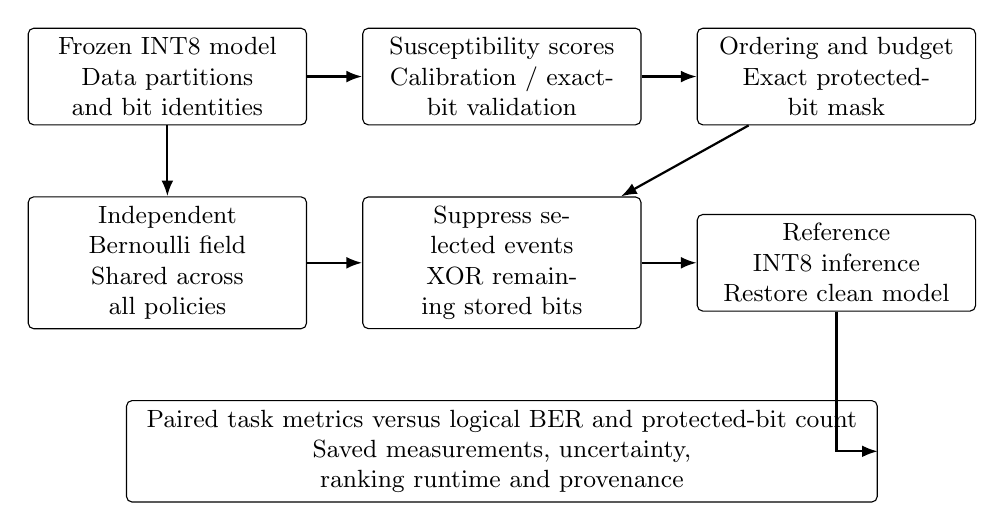
\begin{tikzpicture}[font=\small,box/.style={draw,rounded corners=2pt,align=center,text width=3.3cm,minimum height=1.05cm},arr/.style={-{Latex[length=2mm]},thick}]
\node[box] (frozen) {Frozen INT8 model\\Data partitions and bit identities};
\node[box,right=7mm of frozen] (scores) {Susceptibility scores\\Calibration / exact-bit validation};
\node[box,right=7mm of scores] (mask) {Ordering and budget\\Exact protected-bit mask};
\node[box,below=9mm of frozen] (field) {Independent Bernoulli field\\Shared across all policies};
\node[box,right=7mm of field] (xor) {Suppress selected events\\XOR remaining stored bits};
\node[box,right=7mm of xor] (infer) {Reference INT8 inference\\Restore clean model};
\node[box,below=9mm of xor,text width=9.3cm] (report) {Paired task metrics versus logical BER and protected-bit count\\Saved measurements, uncertainty, ranking runtime and provenance};
\draw[arr] (frozen)--(scores);\draw[arr] (scores)--(mask);
\draw[arr] (frozen)--(field);\draw[arr] (field)--(xor);\draw[arr] (mask)--(xor);
\draw[arr] (xor)--(infer);\draw[arr] (infer.south)|-(report.east);
\end{tikzpicture}

\smallskip
\begin{tabular}{lccc}
\toprule
INT8 example: scale $1/16$, zero point $0$ & Stored word & Decoded value & Exact jump\\
\midrule
Original code $-3$ & \texttt{11111101} & $-0.1875$ & ---\\
Flip least-significant bit & \texttt{11111100} & $-0.2500$ & $-0.0625$\\
Flip sign bit & \texttt{01111101} & $+7.8125$ & $+8.0000$\\
\bottomrule
\end{tabular}
\caption{\textbf{What does a protected bit change?} NetSuRF links a finite stored-code perturbation to a measured task outcome through a matched software experiment. Gradients are ranking surrogates; only the reference interpreter supplies clean and faulted outcomes. The worked INT8 example is analytical, not a sampled model weight. The budget counts selected eligible bits; no physical mitigation or cost is implied.}
\Description{A workflow separates frozen inputs, ranking, a fixed-cardinality mask, shared random fields, exact XOR, and restored reference inference. An INT8 example shows that a near-zero weight can have a large sign-bit jump.}
\label{fig:workflow}
\end{figure}

\section{Exact Encoded-Bit Fault Model}
\label{sec:faults}
Let $\bits$ be the eligible kernel-bit population. A bit is identified by TFLite tensor, flattened word index, and bit position $k\in\{0,\ldots,7\}$, with $k=0$ least significant. Every allocated INT8 kernel word is included, even when its code is zero. INT32 biases, quantization scales and zero points, activations, and operator metadata are excluded. The resulting scope is kernel-storage faults, not all possible model-state faults.

For a signed code $q$, unsigned representation $u=q\bmod256$, scale $s>0$, and zero point $z$, the decoded parameter is $w=s(q-z)$. The numerical effect of flipping bit $b=(q,k)$ is exactly
\begin{equation}
\delta_b=s\left[\operatorname{signed8}\!\left(u\mathbin{\oplus}2^k\right)-q\right].
\label{eq:delta}
\end{equation}
For $k<7$, this equals $s(1-2u_k)2^k$; for $k=7$, it is $-128s(1-2u_7)$. Zero point cancels in the difference, but channel scale does not. Multiple distinct bit changes within one word are combined by XOR, not independent overwrites. Applying the same bit twice cancels. Exact decoding matters especially for sign bits and for tensors with different affine scales. Parameter magnitude alone is therefore not an encoding-aware susceptibility measure.

Each proposed fault field $F\subseteq\bits$ includes coordinates independently with probability $p$. It is sampled once per trial and persists across that trial's inputs. For protection set $P$, the applied field is $F\setminus P$. We record proposed, applied, and suppressed events and require proposed = applied + suppressed. The protected count is $m=|P|$ and coverage is $c=m/|\bits|$. Under this law, expected applied count is $(|\bits|-m)p$. Equal $p$ across networks does not imply equal numbers of corrupted bits. No correlated, fixed-count, adversarial, or transient activation process is inferred from these trials.

This is ideal logical event suppression, not a modeled physical correction
mechanism. For a fixed evaluation cohort, let $R(A)$ be the task risk under
applied set $A$. Expected protected risk is
\begin{equation}
J_p(P)=\E_F[R(F\setminus P)].
\label{eq:risk}
\end{equation}
Classification reports accuracy and cross-entropy separately. ToyCar reports file-level ROC-AUC, with $R=1-\AUC$ for allocation diagnostics. Its reconstruction MSE is a separate surrogate metric. Neither the unit of risk nor its interpretation is pooled across tasks.

All measured outcomes use TensorFlow Lite 2.14.1 \texttt{BUILTIN\_REF}, one interpreter thread and no delegates. Faults change actual model buffers in a private flatbuffer copy. They do not add a quantized delta to an off-lattice floating-point shadow. Clean-state restoration and full-protection equality provide necessary controls; they do not turn the simulated masks into a physical correction mechanism.

\section{Susceptibility Estimation and Budgeted Allocation}
\label{sec:estimators}
Let $\ell_x$ be the ranking loss for calibration input $x$, $g_i(x)=\partial\ell_x/\partial w_i$ the companion gradient for the parameter containing bit $b$, and $\delta_b$ its exact jump from Eq.~\eqref{eq:delta}. We distinguish predicting a signed loss change from ordering bits by a nonnegative score.
Write $z_b(x)=g_i(x)\delta_b$ and $[u]_+=\max(0,u)$.
Table~\ref{tab:definitions} puts each competing score on the same footing;
ordering and budget selection remain separate operations.
\begin{table}[t]\centering\small
\caption{Score definitions and ordering. A score is not a mitigation guarantee or an expected protection benefit. Here $i$ is the parameter containing bit $b$; absolute values on vectors are componentwise.}
\label{tab:definitions}
\begin{tabular}{lll}\toprule
Method & Score or ordering criterion & Ordering\\\midrule
Random & Seeded independent uniform scores & Global\\
MSB-first & Encoded significance $k_b$ & Tier, then identity\\
Numerical jump & $|\delta_b|$ & Global\\
Global gradient & $|\E_x z_b(x)|$ & Global\\
Absolute gradient & $\E_x|z_b(x)|$ & Global\\
Positive gradient & $\E_x\!\left[[z_b(x)]_+\right]$ & Global\\
FKeras~\cite{weng2024fkeras} & $|\sum_j\lambda_j(v_j^\top\theta)v_{ji}|$ & Tier, then score\\
Historical qPolarGrad & $|\E_x[\widetilde a_i(x)\delta_b]\E_x g_i(x)|$ & Historical scope\\
\bottomrule\end{tabular}
\end{table}
The positive-gradient expectation applies \emph{after} taking the positive part
of each example; it is not $[\E_x z_b(x)]_+$. The historical row describes the
recovered dense first-call path, not a new convolutional generalization.

\paragraph{Common static baselines.}
Random assigns reproducible seeded scores over the same eligible population. Corrected MSB-first orders encoded positions $7,6,\ldots,0$, then canonical tensor/word identity. Numerical jump orders $|\delta_b|$ globally. Unlike MSB-first, it includes affine scale differences; unlike a task-sensitive estimator, it does not use input data or loss.

Three first-order scores are
\begin{align}
s_b^{\mathrm{global}}&=\left|\E_x[g_i(x)]\delta_b\right|,\label{eq:global}\\
s_b^{\mathrm{absolute}}&=\E_x\left[|g_i(x)\delta_b|\right],\label{eq:absolute}\\
s_b^{\mathrm{positive}}&=\E_x\left[\max\{0,g_i(x)\delta_b\}\right].\label{eq:positive}
\end{align}
The first retains the magnitude of the mean effect; the second prevents cancellation across examples; the third retains only positive per-example first-order contributions. The signed global approximation is $\E_x[g_i(x)]\delta_b$, without the absolute value. None is an exact finite-bit prediction or a protection benefit. In particular, the positive part of each example's approximation is not the positive part of the aggregate exact damage. Absolute and positive per-example methods share their gradient computation.

These gradients are obtained from architecture-specific companions reconstructed from the frozen constants. Kernel identities, flattened indices, decoded values, and affine metadata correspond to the reference model. Straight-through derivatives pass through activation rounding and clipping, while forward arithmetic does not reproduce all integer multiplier rounding. The classification ranking loss is sparse cross-entropy on companion logits; exact evaluation uses the reference probabilities. ToyCar ranking differentiates float-target reconstruction MSE. Neither the gradient nor the ranking loss is relabeled as a derivative of exact integer inference.

\paragraph{FKeras.}
For decoded kernel vector $\theta$ and leading eigenpairs of a continuous companion loss Hessian, we use the published parameter projection~\cite{weng2024fkeras}
\begin{equation}
h_{\mathrm{FKeras}}=\sum_{j=1}^{k}\lambda_j(v_j^\top\theta)v_j.
\label{eq:fkeras}
\end{equation}
The absolute component $|h_{\mathrm{FKeras},i}|$ orders parameters within each
bit-significance tier. This definition is chosen to represent the published
method, independently of the observed outcomes. Implementation assumptions for
our quantized KWS adaptation are a continuous float64 DS-CNN cross-entropy loss,
without activation requantization; two signed eigenpairs ordered by eigenvalue
magnitude; and canonical tensor/word identity for ties. These choices do not
assert equivalence to every numerical setting of the upstream implementation~\cite{fkerasSource}.
Residual, symmetry, orthogonality and parameter-mapping checks qualify the
bounded eigensolve. Its Hessian is neither an integer-program Hessian nor the
straight-through gradient object above. A full weight Hessian contains mixed
curvature; this clean-point score does not explicitly condition on BER or the
current mask.

FKeras orders bit tiers first and parameter sensitivity within each tier. For $n$ homogeneous INT8 words, any such policy selects all $n$ sign bits at 12.5\% coverage and all sign/bit-6 bits at 25\%. The masks therefore coincide with corrected MSB-first at those budgets, irrespective of the Hessian score. Partial-tier budgets are necessary to test score-dependent allocation decisions. No extra bit-jump multiplier is inserted into FKeras to change this rule.

\paragraph{Historically faithful qPolarGrad.}
The recovered dense first-call implementation ranks approximately
\begin{equation}
s_b^{\mathrm{legacy}}=\left|\E_x[\widetilde a_i(x)\delta_b]\,\E_x[g_i(x)]\right|,
\end{equation}
where downstream inputs
$\widetilde a_i$ come from the historical all-bit-attacked forward state. Its
reproduction removes unintended persistent state accumulation but preserves that
activation source. The rejected manuscript's printed expression appears to
multiply another delta even though its activation-drift term already includes
one; the two are not silently identified. Since a weight gradient already contains
an input factor, the additional activation factor has no automatic first-order
loss interpretation. Clean-activation and magnitude-before-average alternatives
are separately named hypotheses, not a corrected historical method. There is no
validated qPolarGrad pathway or matched efficacy study for the three principal
models here. It is a historical baseline, not an unmeasured curve or headline
contribution.

\paragraph{From scores to a mask.}
Except for tier-first methods, scores are sorted globally with canonical identity
breaking ties. The top $m$ bits form a fixed mask. Random seeds generate distinct
random masks; repeated fields under one mask are not new mask realizations.
The full and zero budgets are shared controls. An exact isolated-bit ranking is
available on explicitly sampled candidates and restricted pools, not over every
bit of all three networks. ``Exact'' describes its measured finite perturbation,
not a universal allocation guarantee.

\section{The Limits of Isolated Bit Rankings}
\label{sec:limits}
For a fixed cohort, isolated damage is $I_b=R(\{b\})-R(\varnothing)$. Define
conditional marginal vulnerability under protected set $P$ as
\begin{equation}
V_b(p,P)=\E_G[R(G\cup\{b\})-R(G)],
\label{eq:conditional}
\end{equation}
where $G$ is Bernoulli over $\bits\setminus(P\cup\{b\})$. Conditioning on the
event at $b$ gives the exact identity
\begin{equation}
J_p(P)-J_p(P\cup\{b\})=pV_b(p,P),\qquad b\notin P.
\label{eq:benefit}
\end{equation}
This is an application of ordinary conditional expectation, closely related to
established importance measures~\cite{odonnell2014analysis,rauzy2022reliability}.
It is valid for a scalar cohort risk, including nonadditive ROC-AUC. It does not
assert that arbitrary faults increase risk, or that protection must always help.

\begin{proposition}
An ordering based only on clean isolated damage does not guarantee an optimal
fixed-cardinality protection mask for arbitrary task-risk functions and
simultaneous independent Bernoulli faults.
\end{proposition}
Consider three bits $a,b,c$ with risks
\begin{center}
\begin{tabular}{c|rrrrrrrr}
$A$ & $\varnothing$ & $a$ & $b$ & $c$ & $ab$ & $ac$ & $bc$ & $abc$\\
\hline
$R(A)$ & 0 & .2 & .1 & 0 & .3 & 0 & .9 & .5
\end{tabular}
\end{center}
Protecting one bit by isolated ranking selects $a$. Exact expectation gives
$J_p(\{a\})=.1p+.8p^2$, whereas $J_p(\{b\})=.2p-.2p^2$. Protecting $b$ is
strictly better for $p>.1$. All responses are bounded in $[0,1]$ and the fault
law is unchanged. The example proves absence of a universal guarantee, not that
every static ranking fails. The deployed optimal mask can itself be static;
the issue is what information was used to construct it. Nor does this example
prove that realistic networks exhibit important allocation regret.

To examine that practical question, we use a deliberately restricted diagnostic.
A candidate set $C$ contains protected and unprotected bits from a verified global
allocation. The external mask $P_{\mathrm{out}}$ is fixed; every candidate choice
$Q\subseteq C$ has the same cardinality. For each sampled outside field $G$, all
$2^{|C|}$ candidate states are evaluated. For a chosen mask,
\begin{equation}
J_p(P_{\mathrm{out}}\cup Q\mid G)=
\sum_{A\subseteq C\setminus Q}p^{|A|}(1-p)^{|C\setminus Q|-|A|}R(G\cup A).
\label{eq:enumeration}
\end{equation}
Candidate integration is exact, including every interaction order in that set;
expectation over outside fields is still estimated. A mask is chosen only on
model-selection data and then compared on independent final fields. Original
gradient allocation, exact isolated allocation, and bounded selected allocation
remain distinct comparators. These are diagnostics of local decisions at a fixed
global budget, not whole-network optimization. The proof and paired-swap identity
are given in Appendix~\ref{app:proof}; the engineering results remain the main
evaluation.

\section{Experimental Methodology}
\label{sec:methods}
\subsection{Frozen models and task metrics}
We use three independently developed MLPerf Tiny reference models~\cite{banbury2021mlperf,mlcommons2026tiny}, without retraining or converting them to a new precision. Each has ten eligible kernel tensors. Table~\ref{tab:models} gives the actual kernel populations and clean quality on the cohorts used for the main static curves. The checkpoints, preprocessing, exact sample indices, backend versions and hashes are bound by the archived manifests. These measurements are not official benchmark submissions or results over every available example.

\begin{table}[t]
\caption{Frozen INT8 benchmarks used for the static protection curves. Kernels only; zero-valued allocated words remain eligible. Clean quality is cohort-specific.}
\label{tab:models}\centering\small
\begin{tabular}{lrrrl}
\toprule
Model / task & Kernel words & Eligible bits & Evaluation cohort & Clean quality\\
\midrule
ResNet-8 / CIFAR-10 & 77,360 & 618,880 & 1,000 images & accuracy .8800\\
DS-CNN / keyword spotting & 22,016 & 176,128 & 1,000 clips & accuracy .9010\\
ToyCar / anomaly detection & 264,192 & 2,113,536 & 64 files & ROC-AUC .86914\\
\bottomrule
\end{tabular}
\end{table}

Classification cross-entropy is $-\log\max(q_y,10^{-12})$, averaged over
inputs, with decoded reference softmax probability $q_y$ and natural logarithm.
The finite floor handles zero output codes; it is not companion-logit loss.
CIFAR-10 inputs use the pinned reference encoding. Keyword spotting uses the
official MFCC pipeline and sample order, including waveform normalization,
16,000-sample clips, 480/320 STFT framing, 40 mel bins and ten coefficients;
an approximate replacement feature pipeline is not used. ToyCar uses the pinned
128-bin log-mel representation, FFT 1024, hop 512, frames 50--250, and five-frame
concatenation, giving 196 windows of 640 features per file. Its preprocessing
also pins the validated two-thread numerical reduction mode; reference inference
remains single-threaded. These numerical details are necessary to reproduce
scores, not incidental implementation choices.

For ToyCar, each reference output is decoded and compared to the original
float-domain feature target. A file score is the mean window reconstruction error.
All windows of all files in a trial share the same faulty model. With anomaly
scores $s_f$, anomaly set $\mathcal D_+$ and normal set $\mathcal D_-$,
\begin{equation}
\AUC=\frac{1}{|\mathcal D_+||\mathcal D_-|}
\sum_{i\in\mathcal D_+}\sum_{j\in\mathcal D_-}
\left[\ind(s_i>s_j)+\tfrac12\ind(s_i=s_j)\right].
\label{eq:auc}
\end{equation}
The main cohort contains 32 normal and 32 anomalous files. We do not calculate
window-level AUC, average per-file AUCs, or treat the pairwise terms in
Eq.~\eqref{eq:auc} as independent observations. Reconstruction MSE remains a
separate ranking/diagnostic objective.

\subsection{Partitions and empirical susceptibility}
Gradient calibration uses 64 training images for ResNet-8 and 64 training clips
for KWS. ToyCar uses 16 complete normal training files, hence 3,136 windows.
Empirical isolated-bit validation uses disjoint calibration-validation inputs:
64 separate training images for ResNet-8, 64 disjoint validation clips for
KWS, and 64 class-containing ToyCar test files disjoint from its final 64-file
cohort. Exact sample identities, not just split names, determine disjointness.
Calibration may be drawn from model-training data; it is not claimed to be a
new held-out generalization set.

Each empirical study samples four bits without replacement from each of ten
kernel-by-eight-position strata: 320 common candidates for all scores. Inclusion
probability is $4/n_t$ in a tensor stratum containing $n_t$ words. This balanced
design is not a uniform sample of all network bits. Each candidate is flipped
alone using the reference interpreter. Signed loss change, its positive part,
absolute change, and accuracy change are retained separately. Spearman uses
average tied ranks; its saved intervals use 1,000 within-stratum bootstrap draws.
Top-$k$ comparisons are restricted to these candidates and account explicitly for
score-boundary ties. They do not estimate whole-network top-$k$ recall.

\subsection{Matched protection studies}
All six common policies use the same checkpoint, eligible universe, calibration,
budget and proposed fields within a study. Interior coverages are 12.5\% and
25\%, with shared zero- and full-protection controls. ResNet-8 and KWS use
$p\in\{10^{-5},10^{-4},3\!\times\!10^{-4},10^{-3},3\!\times\!10^{-3},10^{-2},.03,.1\}$;
ToyCar uses $\{10^{-5},10^{-4},10^{-3},10^{-2}\}$. Larger values are logical stress
conditions. The missing partial-tier and ToyCar intermediate-BER cells are not
interpolated into experimental results.

At each BER, the classifiers have four schedule replications with eight fields
each, for 32 paired fields. ToyCar has two replications with four fields, for
eight paired fields. Random masks are independently constructed once per
replication: there are four classifier masks and two ToyCar masks, not 32 or
eight independent random rankings. Other masks remain fixed. A replication's
seed is distinct from its mask seed. Pairing requires the full BER, replication,
trial and field identity. Full protection must reproduce the corresponding
clean metric and zero protection must suppress no proposed events.

Reported means and descriptive 95\% Student-$t$ intervals use complete fault
trials, not individual inference observations. Policy effects use paired
differences. Saved two-sided sign-flip tests and Holm adjustment retain the
original within-BER, per-metric families; marginal intervals are not simultaneous
intervals and their overlap is not a paired test. Random-policy pooled intervals
condition on the realized masks and do not measure population uncertainty over
new random rankings. Discrete, tied and heavy-tailed outcomes limit small-sample
inference, particularly ToyCar's eight fields.

All numerical evidence comes from finalized bundles. The main figures retain all
methods and measured BERs rather than choosing a favorable model or operating
point. The data have been repeatedly examined during development; the consolidated
comparison is exploratory, even where masks and final schedules were separated
within a particular protocol. No new training or fault campaign was executed to
produce this manuscript.

\section{Results}
\label{sec:results}
\subsection{Do susceptibility scores predict isolated damage?}
Figure~\ref{fig:validity} compares scores with the positive part of exact
isolated loss change. The balanced-stratum associations are positive for most
methods but far from perfect. On ResNet-8, per-example absolute ranking has
Spearman correlation .376, compared with .364 for global first-order and .256
for MSB-first. Numerical jump alone is much weaker (.070). KWS has smaller
associations: .288 for per-example absolute, .258 for global first-order and
.204 for MSB-first. Overlapping candidate-bootstrap intervals do not establish
pairwise estimator superiority; the point estimates describe this sampled design.

ToyCar's positive per-example score has the strongest point association (.637),
followed by per-example absolute (.546) and MSB-first (.502). However, the measured
damage in that panel is reconstruction MSE, not ROC-AUC. It would be a category
error to infer that the best MSE association must give the best anomaly-detection
protection. The random reference's near-zero correlations are from a single
sampled ordering, not a population confidence statement about random policies.
Signed and absolute damage results, tied-score fractions and sample top-$k$
statistics are retained in the evidence supplement rather than collapsed into a
single claim of estimator quality.

\begin{figure}[t]\centering
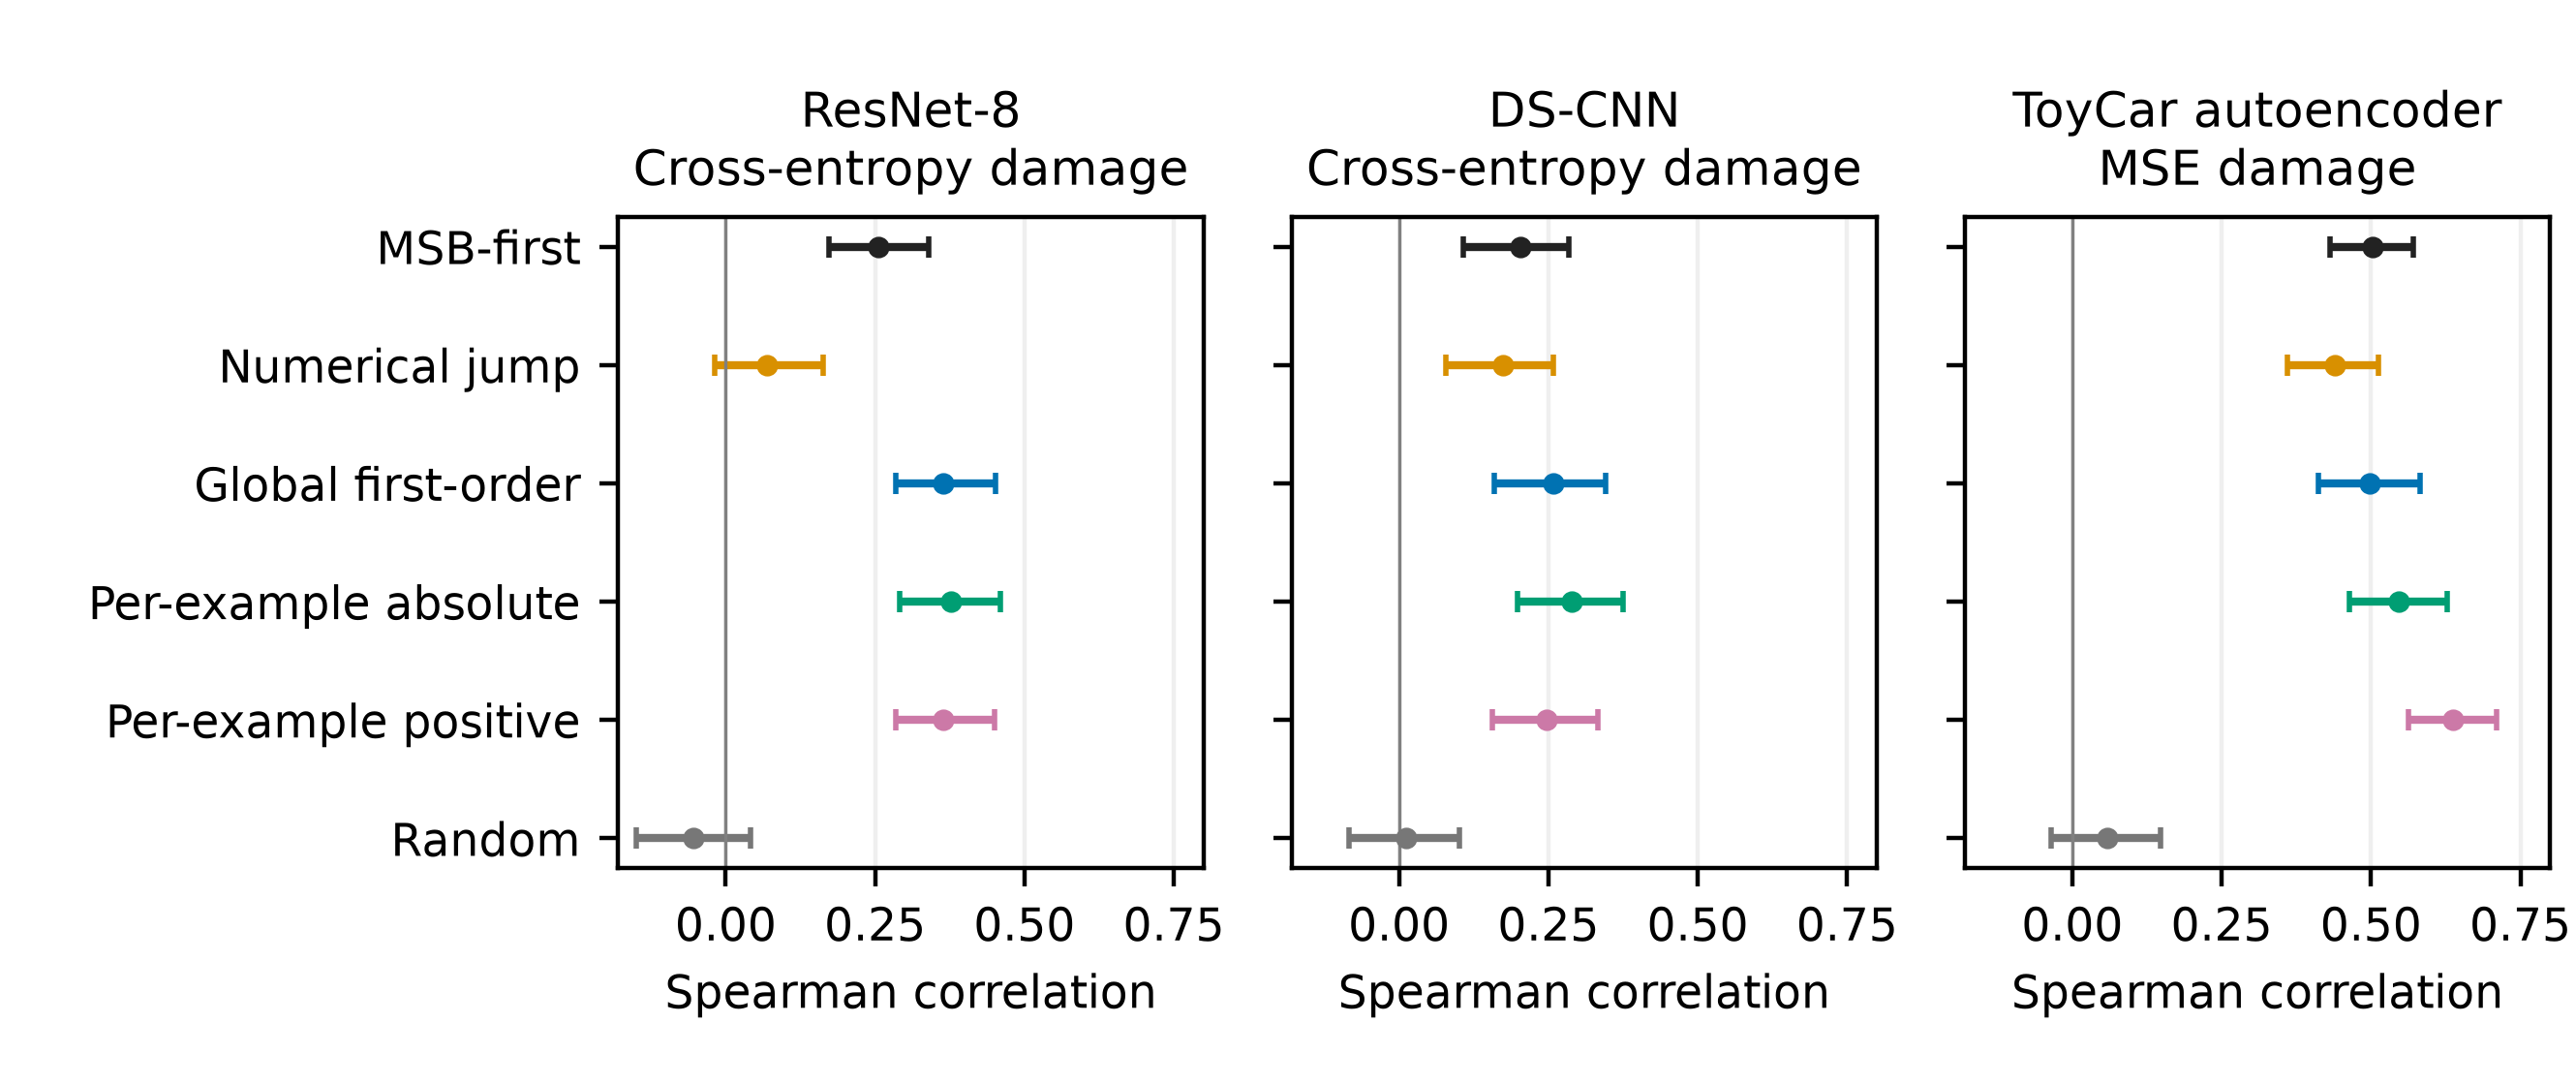
\includegraphics[width=\linewidth]{estimator_validity.png}
\caption{\textbf{How well does a score identify damaging isolated bits?} Spearman association with positive exact loss damage on the same 320 sampled bits per model. Bars are saved 95\% within-stratum candidate-bootstrap intervals. Each of 80 tensor/bit strata contributes four candidates, so these are sample-design results, not whole-network estimates. ToyCar uses MSE damage here; it is not an AUC-validity plot.}
\Description{Three dot-and-interval panels compare six methods. Associations vary by model; ToyCar positive-gradient scores correlate with MSE damage, without establishing AUC protection quality.}
\label{fig:validity}\end{figure}

The companions' numerical limitations are material. The ResNet-8 correspondence
audit identifies class disagreements, not merely different low-order codes.
Kernel mapping is exact; accumulated rounding differences and the final
softmax can amplify small logit differences. Bounded KWS and ToyCar checks also
show nonidentical output codes. Consequently, gradient ranking is defensible as
an empirically tested proxy, not a derivative certificate for the integer program.
These discrepancies are not concealed by substituting the companion for faulted
inference.

\subsection{Reliability versus protection budget}
Figure~\ref{fig:budget} restores the central engineering comparison: what task
quality is retained as the fraction of protected bits increases? All methods
start at the shared unprotected point. Full protection is the deterministic clean
reference, not an interpolated data point between 25\% and 100\%.

At $p=.01$, ResNet-8 accuracy at 12.5\% coverage is .7462 for per-example absolute,
.6402 for global first-order, .4161 for MSB-first, and .1549 for random. At 25\%,
the first two increase to .8205 and .7662, while MSB-first reaches .7537. The
companion proxy thus produces practically different masks with substantial
benefit under these tested conditions. The corresponding cross-entropies also
improve: at 12.5\%, per-example absolute gives 1.7502 versus MSB-first's 8.7914.
This is not solely an accuracy-threshold artifact.

KWS is different. At $p=.01$ and 25\% protection, per-example absolute and
MSB-first give accuracies .8822 and .8802, close to clean .9010; global first-order
gives .8413. Thus the simpler corrected MSB baseline is competitive here. A
more expensive or more task-aware score does not automatically improve the
allocation. At 12.5\%, per-example absolute has a positive paired effect, but
its saved familywise-adjusted test does not cross .05 (Table~\ref{tab:effects}).

ToyCar exposes a stronger objective mismatch. At $p=.01$, MSB-first AUC decreases
from .7101 at 12.5\% coverage to .4327 at 25\%, while its reconstruction MSE
decreases from 240.10 to 203.43. Numerical-jump AUC similarly falls from .7313
to .4197 while MSE improves from 515.56 to 151.87. These are observed means over
only eight fields, not a general claim that protection hurts anomaly detection.
They do demonstrate why the two metrics cannot be substituted for one another.
At 25\%, per-example absolute's AUC is .6742, yet global first-order and random
have higher point means (.7185 and .6849); uncertainty remains substantial.

\begin{figure}[p]\centering
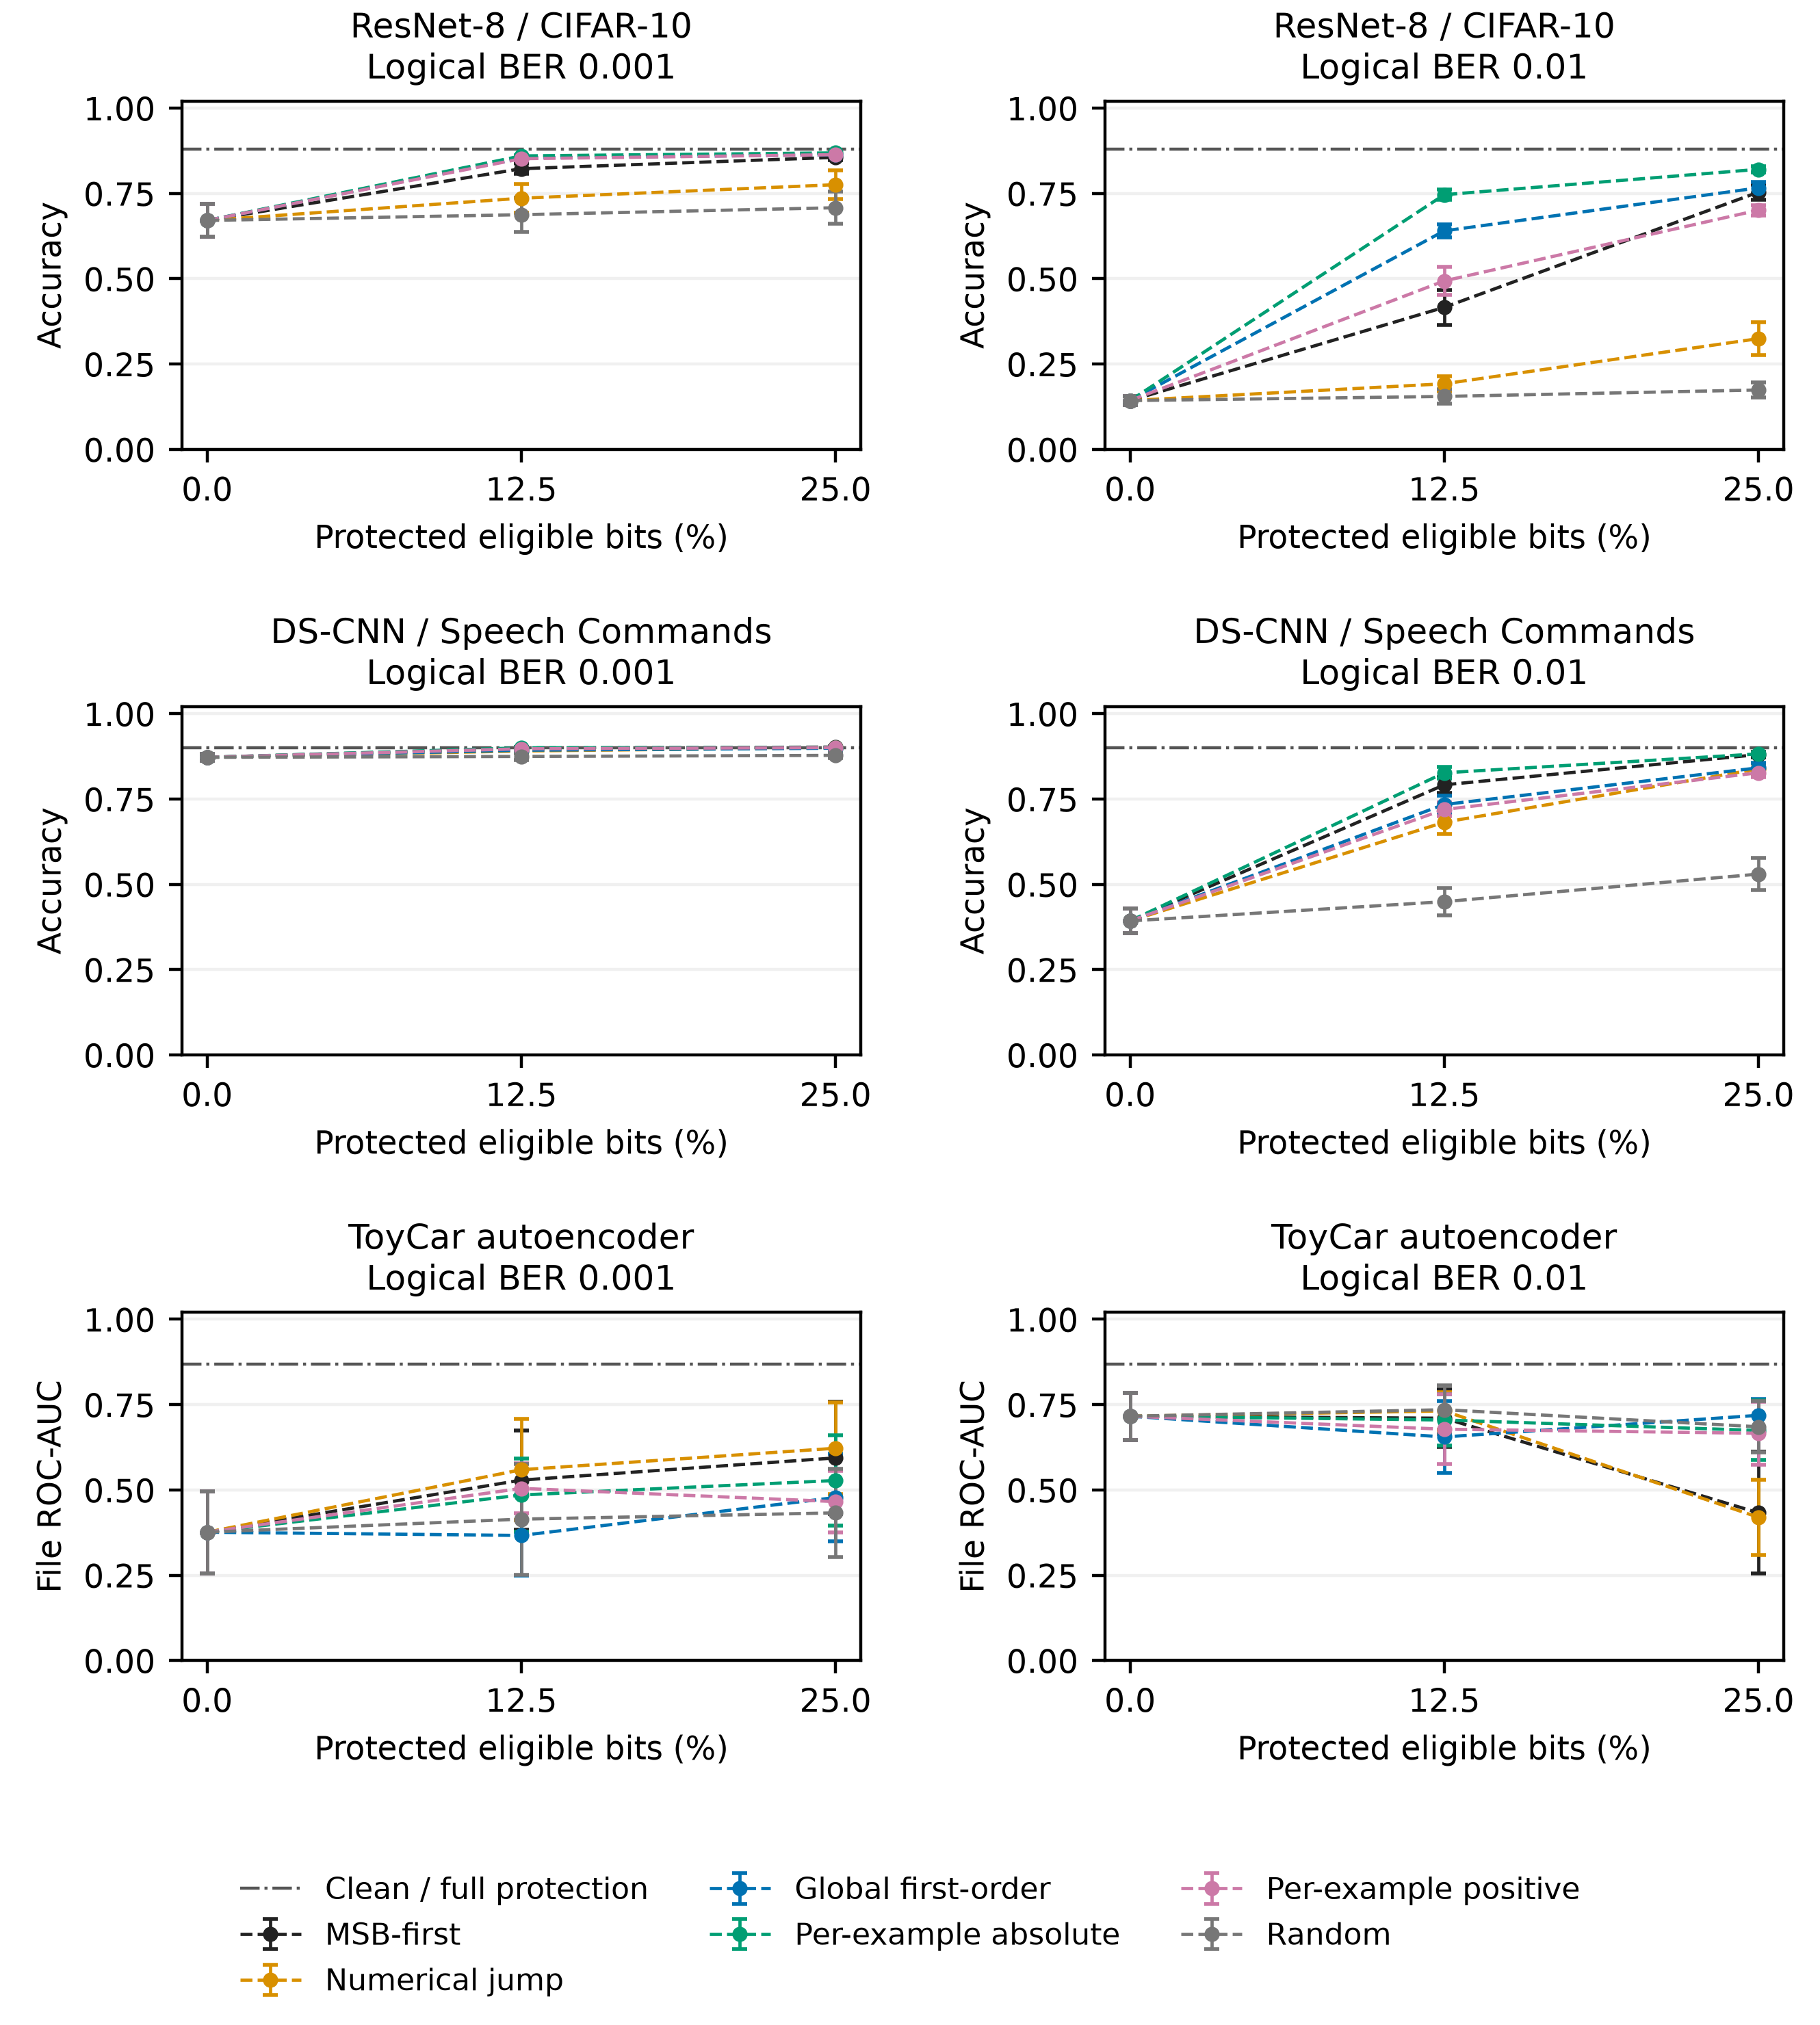
\includegraphics[width=.98\linewidth]{protection_budget.png}
\caption{\textbf{How much task quality does a logical protection budget preserve?} All six policies at matched BER .001 and .01. ResNet-8 and KWS have 32 paired fields per BER; ToyCar has eight. Points are observed coverages only (0, 12.5\%, 25\%); dashed segments are guides, not fitted response models. Bars are descriptive 95\% field-$t$ intervals intersected with $[0,1]$, conditional on the fixed cohort and realized masks. Random-mask variability is nested by replication. No 6.25\% or 18.75\% effectiveness measurements are implied.}
\Description{Six panels show accuracy or file AUC against protected-bit fraction. ResNet improves strongly with gradient masks, KWS MSB is competitive, and ToyCar exhibits nonmonotonic and uncertain budget effects.}
\label{fig:budget}\end{figure}

\begin{table}[t]\centering\small
\caption{Paired per-example absolute minus MSB-first effects at BER .01, both budgets and all three tasks. Accuracy differences are percentage points (pp); ToyCar differences are AUC units. Intervals are marginal field-$t$ intervals. Holm values retain the source's within-BER/metric comparison family, not a new family selected from these six rows.}
\label{tab:effects}
\begin{tabular}{lrrrrr}
\toprule Task / units & Budget & Fields & Mean & 95\% interval & Holm $p$\\\midrule
\tablerows{tables/paired_effects.tex}
\bottomrule\end{tabular}
\end{table}

Table~\ref{tab:effects} illustrates why interval direction and adjusted tests must
be reported together. ResNet effects are large under this stress condition.
KWS's 25\% effect is small and unresolved. ToyCar's 12.5\% effect is negative
and unresolved; its positive 25\% marginal interval still has Holm-adjusted
$p=.8438$. These statements concern the recorded family and fixed cohorts.
They do not imply a fresh confirmatory test or a universal method ordering.

\subsection{Reliability versus logical BER}
Figure~\ref{fig:ber} retains every measured BER, including saturation regimes.
For the classifiers, small BERs give limited separation because all masks retain
quality near clean inference. Differences become visible as multiple errors
accumulate. At the highest stress conditions, even protected inference can
degrade markedly. KWS at 25\% coverage illustrates an ordering change: MSB-first
and per-example absolute remain close over much of the curve, and MSB-first has
the higher point mean at the largest BER. The paper does not choose one BER
afterward to declare a winner.

ToyCar's AUC is nonmonotonic in BER as well as budget, with low means around
$10^{-3}$ and higher means at $10^{-2}$ for several policies. Reconstruction
error alone cannot explain that trajectory: AUC depends on the relative ordering
of normal and anomalous file scores. Finite fields and a fixed cohort are also
limitations. The data do not identify a causal mechanism or justify assuming a
monotone risk curve. Supplementary loss curves preserve this distinction.

Absolute exposure differs greatly across models. At $p=.001$, expected
unprotected flips are 618.88 for ResNet-8, 176.128 for KWS, and 2,113.536 for
ToyCar. Protection of 25\% of the eligible bits reduces each expectation by
one quarter, but does not equalize it. These facts prevent interpreting
cross-architecture curve separation as a controlled causal comparison of
architectural redundancy.

\begin{figure}[p]\centering
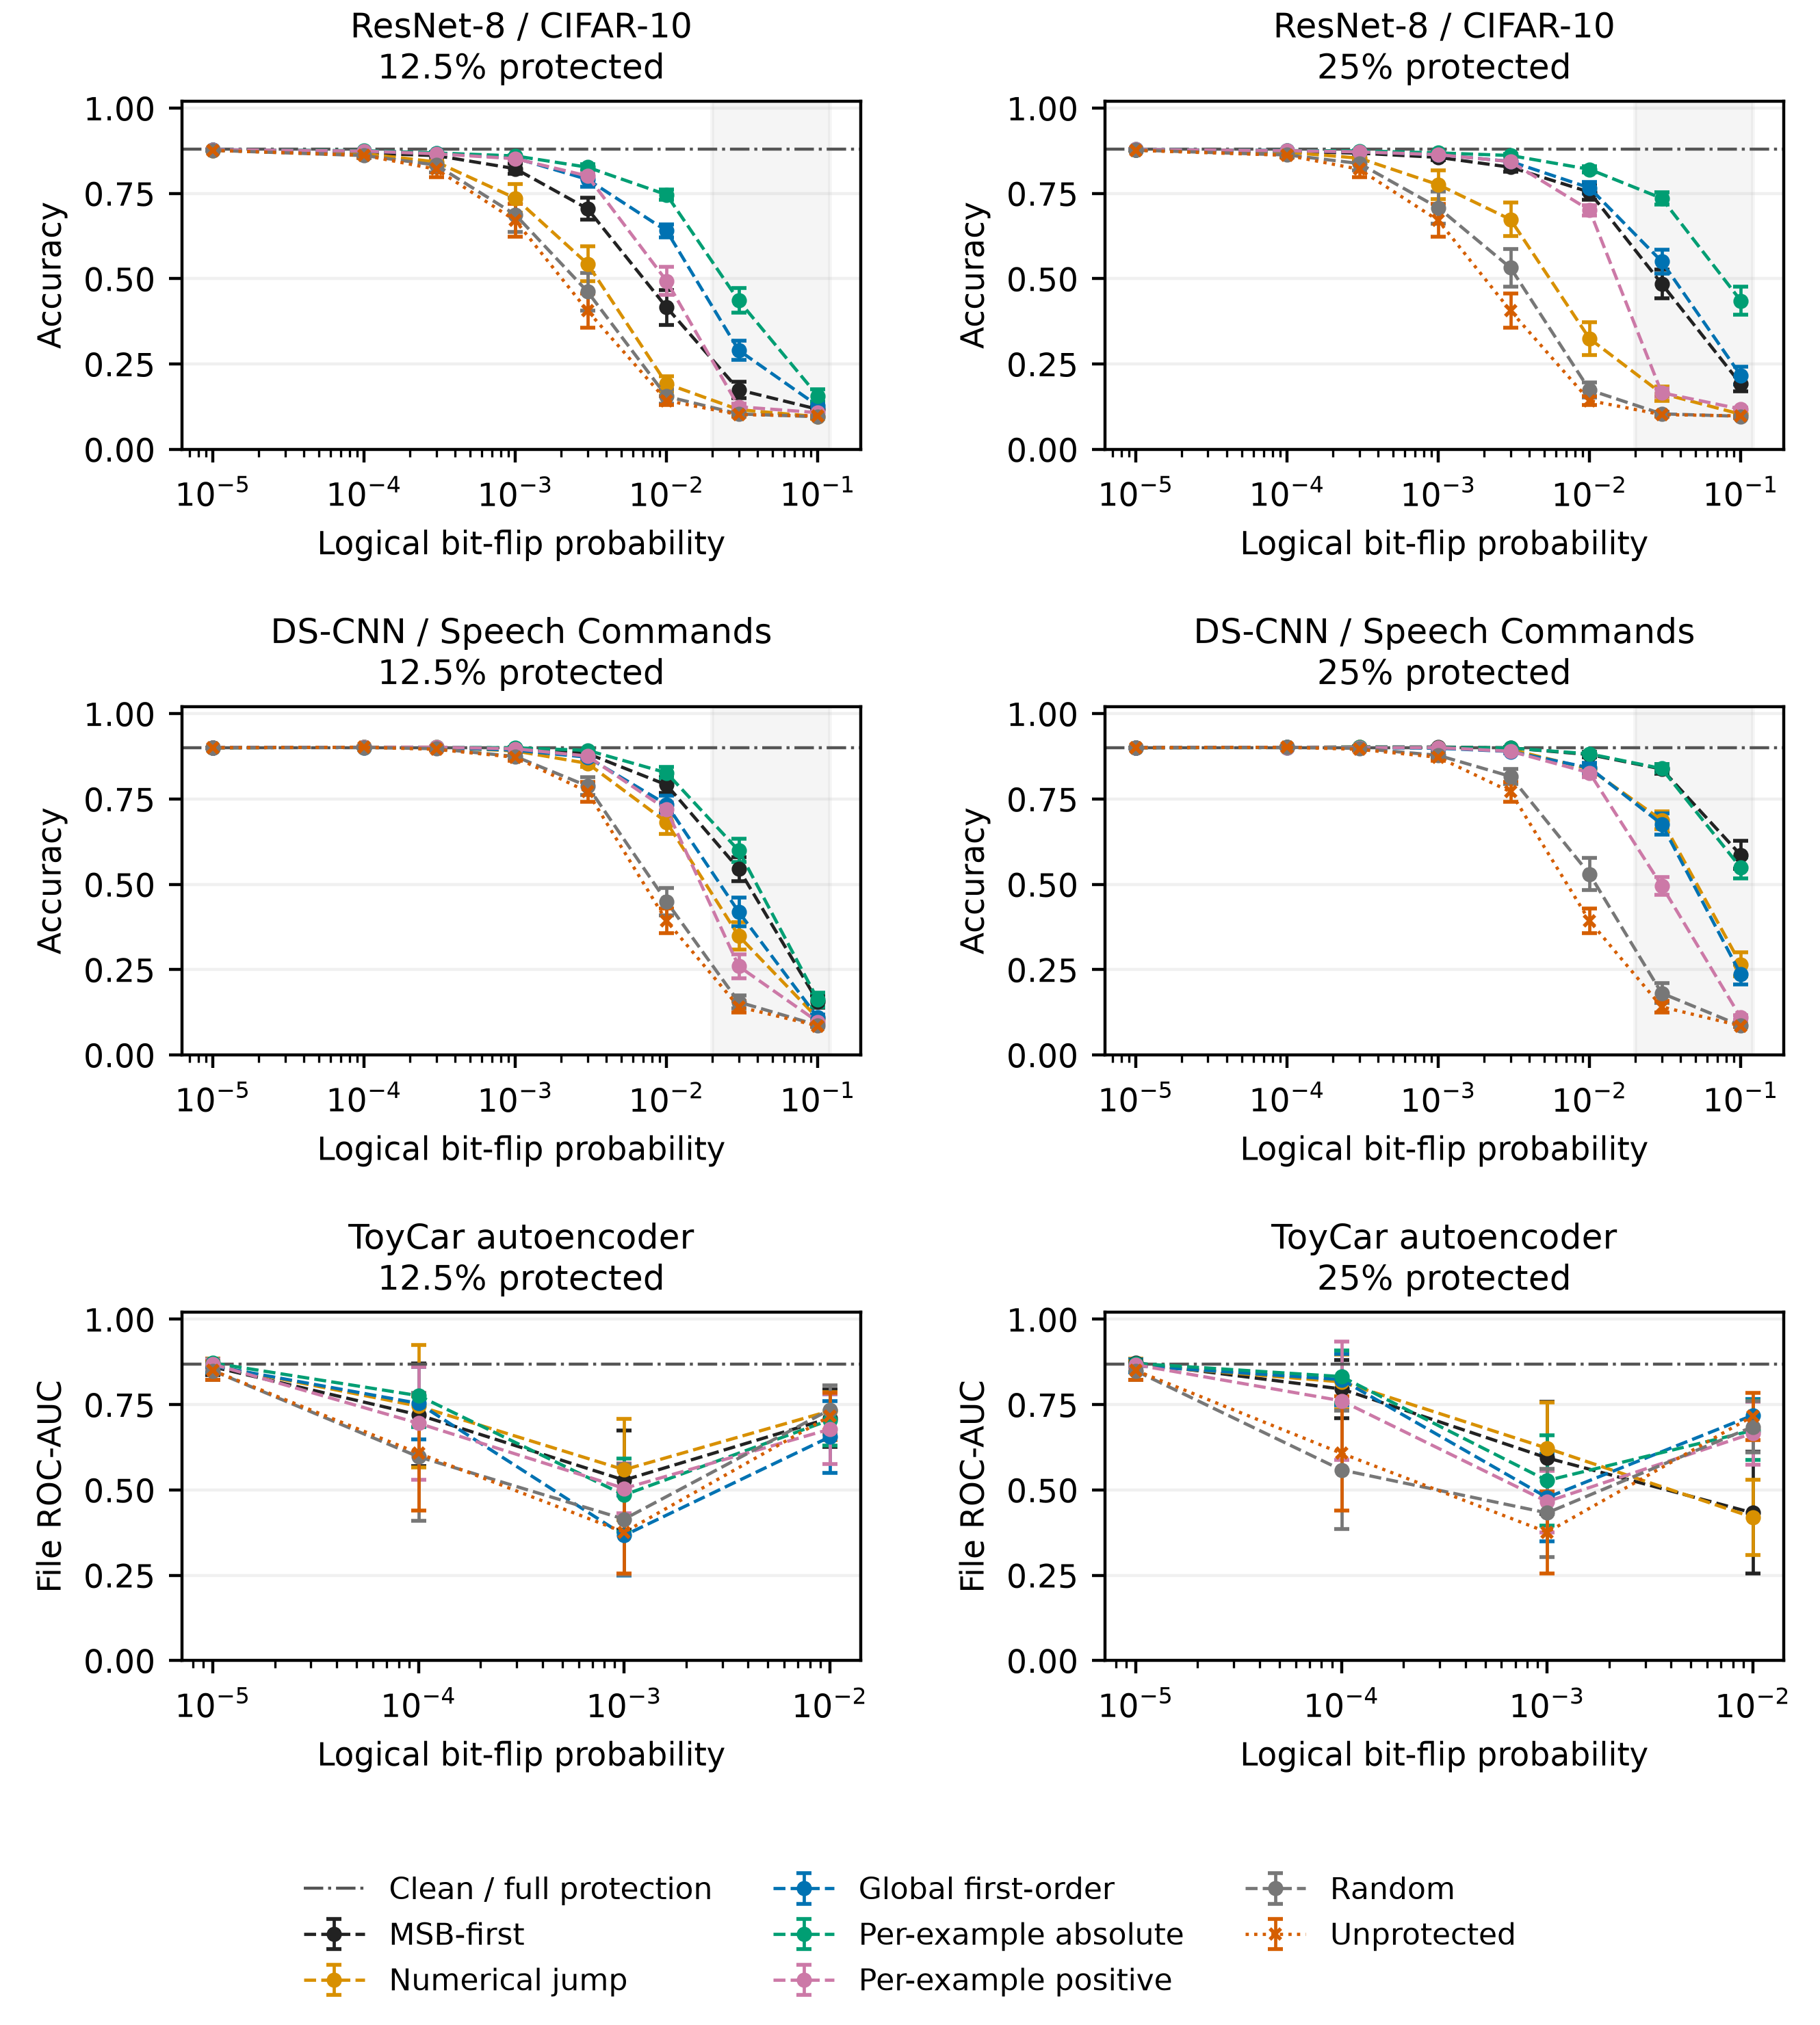
\includegraphics[width=.98\linewidth]{protection_ber.png}
\caption{\textbf{Where does a ranking remain useful as fault probability increases?} Complete measured BER grids at 12.5\% and 25\% coverage. All policies share the same proposed fields within each BER. The horizontal line is clean/full protection; orange crosses are unprotected inference. Larger classifier BERs are shaded as stress conditions. Error bars have the same fixed-cohort interpretation as Fig.~\ref{fig:budget}; the horizontal axis is a logical per-bit probability, not a physical incidence rate. ToyCar has no measured .003, .03 or .1 point in this static study.}
\Description{Six panels plot task quality against logarithmic logical BER, retaining all policies, clean controls, unprotected outcomes, uncertainty and high-BER stress points.}
\label{fig:ber}\end{figure}

\subsection{What the FKeras validation does and does not establish}
The KWS engineering validation uses two calibration clips, four evaluation clips
and two fault fields. Two eigenpairs pass normalized residual and orthogonality
checks, and the two formulas generate different partial-tier masks
(Table~\ref{tab:fkeras}). All protection conditions have accuracy 1.0 in that
small test. This validates execution and mapping, not comparative protection
efficacy. Adding indistinguishable full-tier FKeras curves to the main figures
would not supply an independent baseline.

\begin{table}[t]\centering\small
\caption{FKeras KWS mask validation: symmetric-difference bit counts between saved masks. Complete tiers yield identical sets. Partial tiers expose real formula/tie-order differences but currently lack a meaningful effectiveness study.}
\label{tab:fkeras}
\begin{tabular}{rrrrr}\toprule
Coverage & Protected bits & Paper / repository & MSB / paper & MSB / repository\\\midrule
\tablerows{tables/fkeras_masks.tex}
\bottomrule\end{tabular}
\end{table}

The printed and repository formulations are therefore both retained as validated
score-level baselines with a bounded execution check. An adequately sampled
partial-tier comparison is a missing experimental result, not a reason to
redefine FKeras as global gradient-style ordering or infer that it loses.
Historical qPolarGrad remains outside the principal curves for the analogous
reason: no validated comparable result exists on these three models.

\subsection{Do conditional changes materially improve allocation?}
Conditional diagnostics establish more than the counterexample alone, but less
than a generally effective optimizer. A ten-candidate KWS audit recorded 15 of
45 strict isolated/conditional pair reversals on held-out clips at $p=.001$,
and 18 of 45 at $p=.01$. Shared candidate pairs are not independent trials;
reversals by themselves do not quantify mask regret. An earlier eight-bit
exploratory pool, kept frozen in a 256-field replication, favored selected over
isolated allocation by $-3.810\times10^{-4}$ CE, with marginal interval
$[-4.403,-3.217]\times10^{-4}$. That pool had been historically selected, so
independent final fields do not remove its pool-selection bias.

Figure~\ref{fig:conditional} gives the stronger independent-pool evidence without
selecting favorable pools. Six-bit pools contain two protected and four
unprotected bits sampled within original-mask status strata. All compared masks
retain the global budget. There are 12 pools per KWS arm and four each for
ResNet-8 and ToyCar; the three common-pool KWS BER arms reuse the same pools.
The selected masks improve the point mean relative to the original
per-example absolute allocation in the KWS arms, but \emph{all six
selected-minus-exact-isolated pool intervals include zero}. ResNet-8 and ToyCar
point means against isolated allocation are slightly unfavorable. Pool-level
uncertainty is distinct from field uncertainty and is conditional on a shared
input cohort. The diagnostic therefore limits claims of practical conditional
advantage instead of supplying the main paper's superiority claim.

\begin{figure}[t]\centering
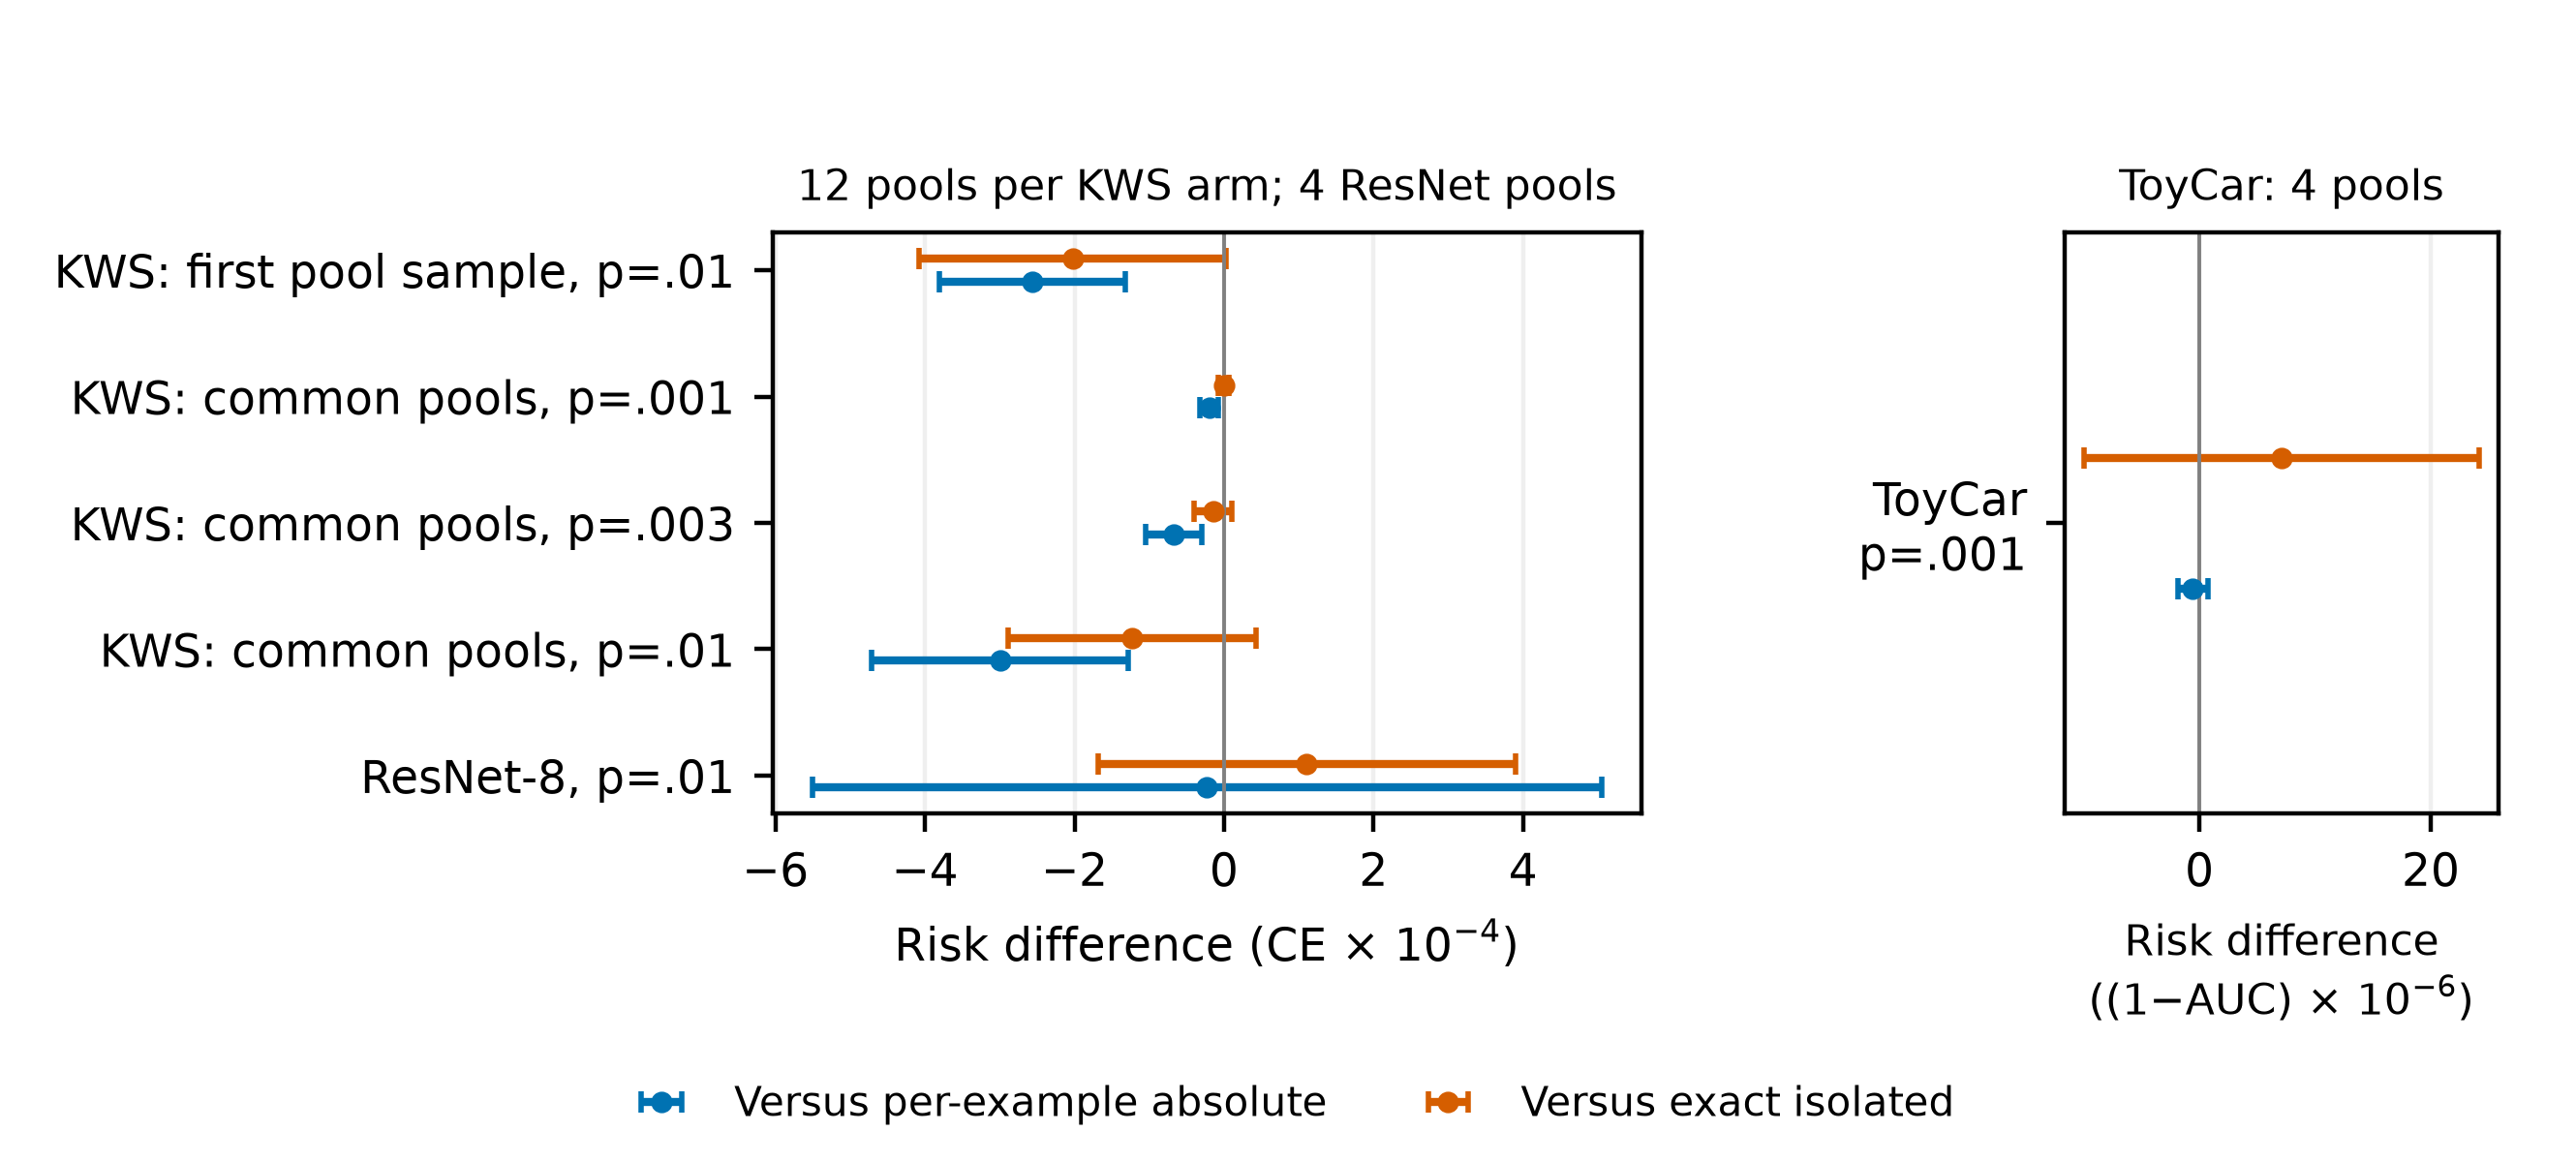
\includegraphics[width=\linewidth]{conditional_limits.png}
\caption{\textbf{Do context-aware local choices improve held-out risk?} Equal-pool mean differences for bounded selected masks against two frozen comparators. Negative favors the selected mask. Bars are marginal 95\% pool-$t$ intervals; common-pool KWS arms are not independent pool samples. Cross-entropy and $1-\mathrm{AUC}$ have separate axes and units. Every independent-pool arm is shown, including zero-crossing and unfavorable effects. These are local equal-global-budget exchanges, not whole-network optima.}
\Description{A forest plot shows selected-minus-gradient and selected-minus-isolated risk differences across all six study arms. Every interval for comparison with exact isolated allocation includes zero.}
\label{fig:conditional}\end{figure}

\subsection{Computation and evidence cost}
\begin{table}[t]\centering\small
\caption{Recorded score-construction time (seconds) in the 320-candidate validation studies. Scores cover the eligible populations. Per-example absolute/positive share computation; the shared time is counted once. Classifiers use 64 calibration examples; ToyCar uses 16 files / 3,136 windows. These are configuration-specific observations, not portable speedups.}
\label{tab:costs}
\begin{tabular}{lrrr}\toprule
Model & Numerical jump & Global first-order & Shared per-example\\\midrule
\tablerows{tables/ranking_costs.tex}
\bottomrule\end{tabular}
\end{table}
Global first-order requires aggregate differentiation, whereas per-example
statistics require retaining signs or magnitudes before reduction. The latter
costs more in every recorded study (Table~\ref{tab:costs}). ToyCar's much larger
calibration-window count is essential context for its 205.88-second shared cost.
Recorded zero timers for simple baselines are not evidence of zero execution
cost and are not used for speedup ratios. The tiny FKeras smoke records 1.12
seconds for a shared eigensolve; that cannot be extrapolated as a fair comparison
with 64-example gradient calibration.

The complete static classifier grids contain 3,584 cohort evaluations each;
ToyCar has 448. Recorded coordinator elapsed times are about 200.3, 45.0 and
21.5 minutes for ResNet-8, KWS and ToyCar, with two, four and two effective
workers respectively. Their bundles occupy approximately 2.50, .72 and 4.04 GB.
These include setup, evaluation and evidence handling, not just ranking.
Large exact score/mask records make ToyCar storage substantial despite fewer
fields. Exact candidate tables cost $2^K$ cohort evaluations per outside field;
using $K=6$ limits this factor to 64 but says nothing about tractability of
whole-network exact allocation. Computation and statistical resolution must be
weighed together before expanding these diagnostics.

\section{Discussion and Validity Boundaries}
The experiments support a decision procedure, not a universal ranker: define the
exact storage population and task metric; test a small set of inexpensive
baselines; compare actual masks at relevant budgets under paired fields; and
spend additional computation only where measurable task benefit warrants it.
For the tested ResNet-8, per-example absolute gradients are useful allocation
proxies at several stress conditions. For KWS, corrected MSB-first is a strong
competitor, especially when a larger budget protects complete significant tiers.
For ToyCar, reconstruction sensitivity must be checked against file ordering;
good MSE prediction alone is inadequate evidence for AUC protection.

Several noncausal explanations remain possible. Gradient cancellation can
separate global and per-example scores, affine scales can separate numerical
jump from MSB ordering, and nonlinear inference can separate isolated damage
from multi-fault benefit. None of these facts identifies the dominant cause of
the cross-model results. The models differ in task, parameters, exposure count,
input distributions and surrogate quality. Weight sparsity is not a measured
causal explanation of redundancy, and the current study does not intervene on
architecture or retrain matched checkpoints.

Only one frozen checkpoint per architecture is evaluated. Fixed-cohort field
intervals do not describe variation over new models or new input populations.
The balanced candidate sample is small within each stratum. ToyCar has few
fault fields and an exposure ledger showing prior clean evaluation of all 248
official files and prior fault-outcome exposure of 200; the remaining 40 normal
and eight anomalous files do not provide a large balanced untouched cohort.
Further trials can improve Monte Carlo precision on reused inputs but cannot
create new input-level confirmation.

The static budget grid has only two interior points. A fair partial-tier
FKeras comparison remains the most consequential baseline gap. Surrogate
gradients are not integer-program derivatives, and the FKeras continuous
Hessian is a third, explicitly different numerical object. Exact isolated
measurements reduce ambiguity about finite effects but still do not certify
multi-fault allocation. Bounded conditional experiments address that distinction
locally; their uncertain and small gains against isolated allocation do not
justify claiming an effective general optimizer.

Finally, logical protected-bit count is deliberately the sole protection cost.
No area, power, energy, latency, synthesis or radiation-calibrated reliability
estimate follows from these software results. Runtime measurements concern the
analysis itself. Excluded biases, metadata and activations remain outside the
fault model rather than being declared universally safe. This restricted scope
makes the comparison auditable, but limits its transfer to other fault domains.

\section{Conclusion}
NetSuRF connects exact INT8 kernel-bit faults to budgeted logical protection and
task-level evaluation through a reproducible software flow. On the three tested
models, ranking quality is not a single property: association with isolated
damage, protection benefit, and computation cost can disagree. Per-example
absolute gradients improve several ResNet-8 allocations; KWS often admits a
competitive MSB baseline; ToyCar demonstrates why reconstruction-MSE sensitivity
cannot substitute for file-level AUC evidence. FKeras's strict bit-tier ordering
also shows why different scores need not produce different masks.

An exact counterexample establishes that isolated susceptibility has no universal
optimal-protection guarantee under simultaneous faults. The independent-pool
measurements do not, however, resolve a practical advantage of bounded
conditional selection over exact isolated allocation. Together, these positive,
negative and unresolved results support NetSuRF as a software methodology for
testing the reliability of ranking-driven decisions, not a universally superior
score or optimizer. Stronger partial-tier baselines, additional fault fields and
independent task populations are the next empirical steps; no physical mitigation
performance is claimed.

\appendix
\section{Conditional Identity and Approximation Limits}
\label{app:proof}
Write $F\setminus P=G\cup B$, where $B$ is either $\varnothing$ or $\{b\}$,
independently of $G$. Then
$J_p(P)=(1-p)\E R(G)+p\E R(G\cup\{b\})$, while
$J_p(P\cup\{b\})=\E R(G)$. Subtraction proves Eq.~\eqref{eq:benefit} without
smoothness or additive-loss assumptions. Setting all outside probabilities to
zero reduces $V_b$ to $I_b$; this special case is not the general multi-fault
objective. Exact enumeration of the eight states in Section~\ref{sec:limits}
gives $J_p(\{a\})-J_p(\{b\})=p(p-.1)$, proving the counterexample.

For an equal-budget exchange, let $a\in P$, $b\notin P$ and
$P'=P\setminus\{a\}\cup\{b\}$. Sample $G$ over all other unprotected coordinates,
excluding $a,b$. The exact identity is
\begin{equation}
J_p(P')-J_p(P)=p\E_G[R(G\cup\{a\})-R(G\cup\{b\})].
\end{equation}
A deterministic path of legal exchanges can compare frozen masks. Contributions
along a path share a master field and are summed before computing uncertainty;
path steps are not independent replications. The identity applies to complete-file
ROC-AUC risk because it only requires a scalar response. It does not require, or
permit substituting, an additive per-window loss.

If an approximate risk table is uniformly within $\epsilon$ of the exact table
over the admissible masks, its minimizing mask has regret at most $2\epsilon$:
compare approximate and exact risks at the approximate and exact minimizers,
and use the approximate minimizer's inequality between them. This elementary
bound distinguishes numerical approximation error from Monte Carlo selection
error. A sum of absolute omitted interaction terms can upper-bound a polynomial
remainder, but at large candidate dimension such worst-case bounds can be
vacuous. Bounded numerical checks do not establish scalable selection benefit.
The Boolean/multilinear foundations are standard~\cite{odonnell2014analysis};
we do not present an unexecuted spectral program as an empirical contribution.

\section{Auxiliary Losses and Reproducibility}
\begin{figure}[p]\centering
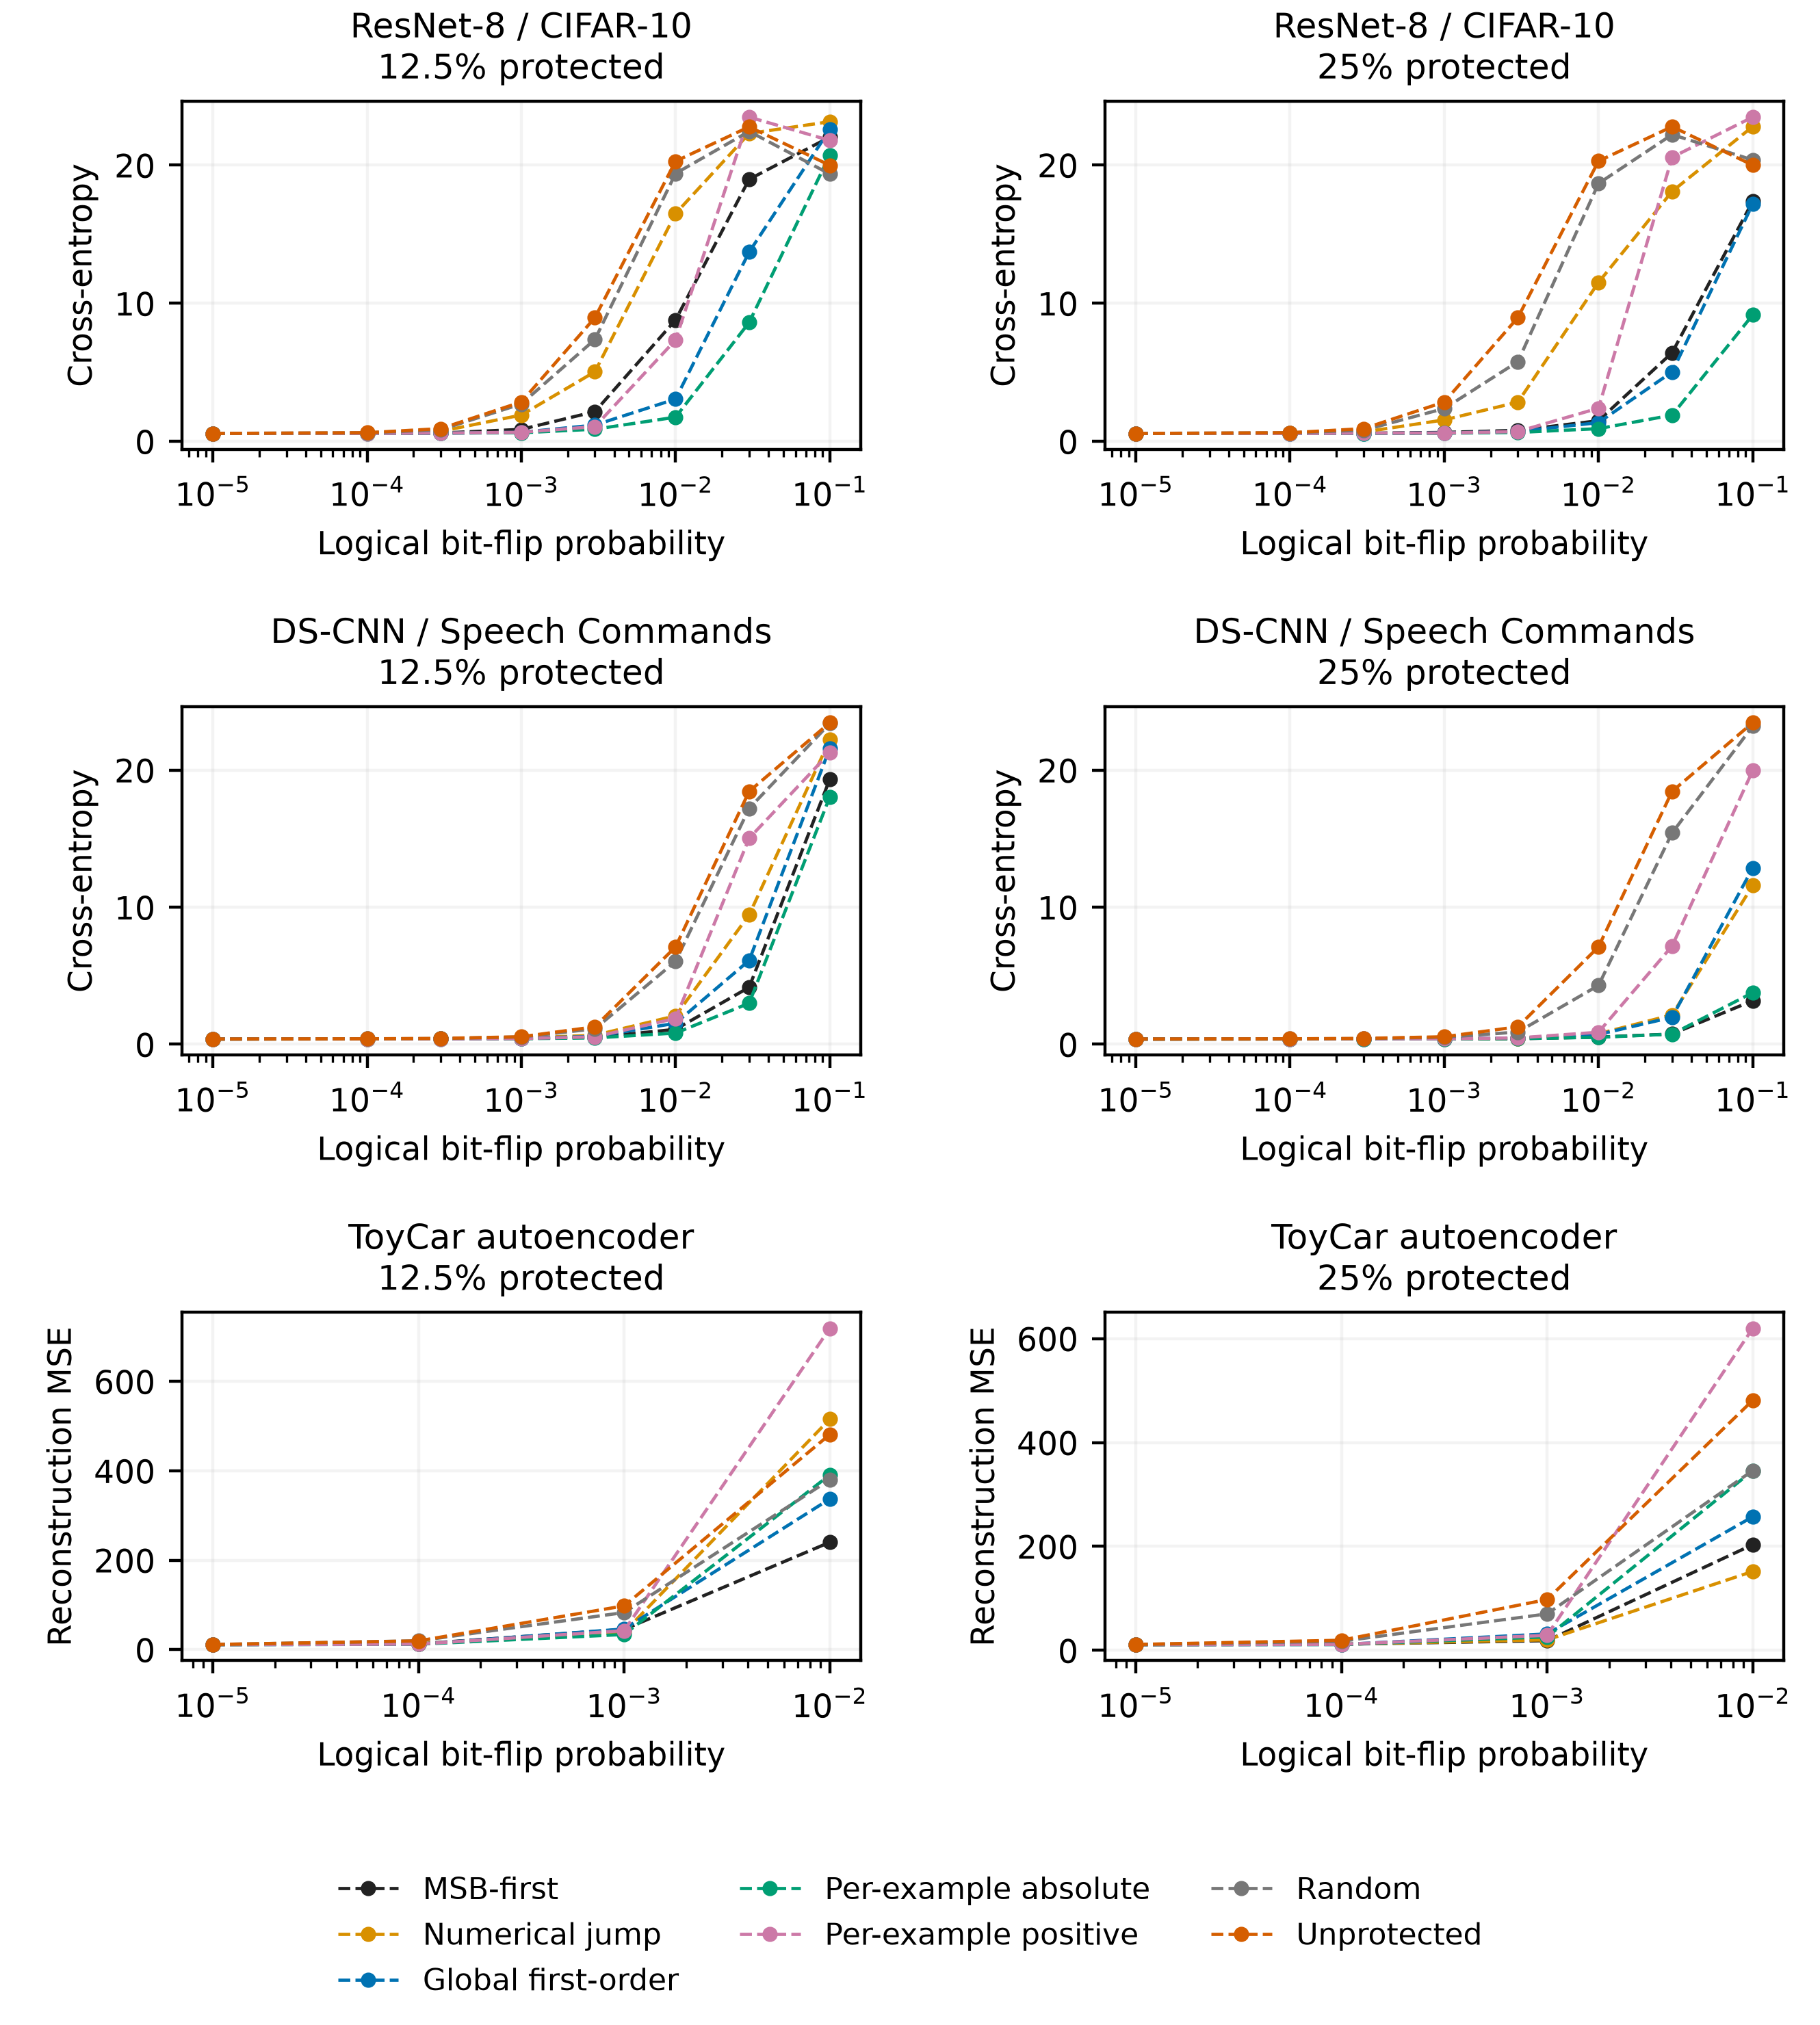
\includegraphics[width=.98\linewidth]{loss_ber.png}
\caption{\textbf{Does the auxiliary loss tell the same story as task quality?} Mean exact reference cross-entropy for the two classifiers and reconstruction MSE for ToyCar across all measured BERs. Units remain separate; no cross-task averaging is performed. The companion loss is used only for ranking. These curves show means; the accompanying numerical supplement retains per-condition standard deviations, standard errors through sample counts, and field-$t$ intervals. In particular, reduced ToyCar MSE need not improve file ROC-AUC.}
\Description{Six auxiliary-loss panels retain all six policies and unprotected controls. ToyCar reconstruction-error trends differ from its file-level AUC trends.}
\label{fig:loss}\end{figure}

The supplementary evidence package contains exact checkpoint and sample
identities, source payload and artifact hashes, raw-derived condition tables,
paired comparisons, figure/table recipes, and the archived method definitions.
Publication figures are generated only from verified finalized measurements.
The audit rechecked 126 finalized records and 612 consumed files, recomputed
10,112 static trial rows into 358 condition summaries, and checked 2,184 paired
summary means and intervals. This scope does not assert that every unused file
in every historical directory was rehashed. Exact masks were hash-verified;
their large files were not re-enumerated during manuscript assembly.

Candidate correlations, pool-level intervals and field-level intervals retain
different sampling units. Ranking masks remain tied to their own construction
seeds. The frozen checkpoints are not retrained for a presentation change.
Original bundles are unchanged, and supplementary figures and tables do not
constitute new scientific trials. The build instructions separate offline
evidence processing from model execution and give the pinned source/backend
requirements for locating the original runs.

\bibliographystyle{ACM-Reference-Format}
\bibliography{references}
\end{document}
